
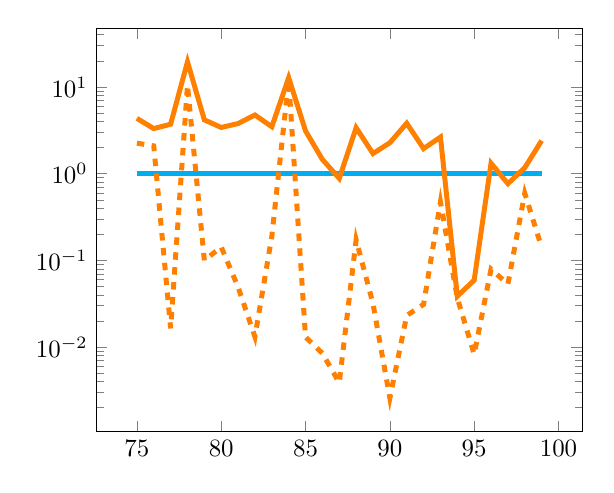
\begin{tikzpicture}[scale=0.9]
\begin{semilogyaxis}
\addplot[color=cyan,line width=2pt] coordinates {(75,1.0)(76,1.0)(77,1.0)(78,1.0)(79,1.0)(80,1.0)(81,1.0)(82,1.0)(83,1.0)(84,1.0)(85,1.0)(86,1.0)(87,1.0)(88,1.0)(89,1.0)(90,1.0)(91,1.0)(92,1.0)(93,1.0)(94,1.0)(95,1.0)(96,1.0)(97,1.0)(98,1.0)(99,1.0)};
\addplot[color=orange,line width=2pt] coordinates {(75,4.343245480839145)(76,3.311755970051883)(77,3.7199759272057995)(78,19.507202736114724)(79,4.173409115213757)(80,3.4116218830082556)(81,3.784722751066593)(82,4.750487411867719)(83,3.4779477963447736)(84,12.790722031014885)(85,3.114025451466972)(86,1.4579101945540702)(87,0.8818012811880485)(88,3.3869827721355468)(89,1.7065719767276464)(90,2.2719840241720495)(91,3.814743601922505)(92,1.9445361014412699)(93,2.6408269371240785)(94,0.03858314348100641)(95,0.05923323450558558)(96,1.3206838200166469)(97,0.7671565246273964)(98,1.1701986627414054)(99,2.4027745621869783)};
\addplot[dashed,color=orange,line width=2pt] coordinates {(75,2.2482235616579875)(76,2.090931854399491)(77,0.01648464850630347)(78,10.510980373464369)(79,0.0997498128256471)(80,0.14310285741063075)(81,0.04928018079999299)(82,0.013173448763109216)(83,0.18931994176986294)(84,12.015016931621794)(85,0.013049321282430686)(86,0.008477983198919396)(87,0.0038839580086849905)(88,0.17309279040078834)(89,0.031708408646990864)(90,0.002588156700417884)(91,0.02317379392288269)(92,0.031068968630790433)(93,0.4722068995500428)(94,0.036909597685447534)(95,0.008270429201323667)(96,0.0792409776707787)(97,0.053198658188827644)(98,0.595883078967837)(99,0.14118995753305782)};

\end{semilogyaxis}
\end{tikzpicture}
